\documentclass[12pt, a4paper]{article}
\usepackage{CJKutf8}
\usepackage[left=2cm, right=2cm, top=3cm, bottom=2.5cm]{geometry}
\usepackage[nodayofweek,level]{datetime}
\usepackage{comment}

%..This section controls the header-footer layout of the document
\usepackage{fancyhdr}
\pagestyle{fancy}
\lhead{Machine Learning (NTU CSIE, Fall 2017)}
\chead{}
\rhead{Instructor: Hsuan-Tien Lin}
\renewcommand{\headrulewidth}{0.4pt}

%..This section controls the title layout
\title{\vspace{-4ex}\bf{\LARGE{Homework \#4}}} 
\author{資工三\space\space\space B04902009\space\space\space 蕭千惠} % \footnote{blablabla} 
\date{\vspace{-2ex}\today\vspace{-4ex}}
%{\formatdate{21}{2}{2017}}

%.. math
\usepackage{mathtools}
\usepackage{amssymb}
\usepackage{amsmath}
\usepackage{upgreek}
\usepackage{bm}

%.. hyperlink / url
\usepackage[hyphens]{url}
\usepackage{hyperref}
\hypersetup{
    colorlinks=true,
    linkcolor=blue,
    filecolor=magenta,      
    urlcolor=blue,
}
\urlstyle{same}
%%\url{url}
%%\herf{url}{words to show}

% .. Include graph
\usepackage{graphicx}
% \includegraphics[width=16.5cm, keepaspectratio=true]{wireless_CSIE_server.png} \par

%.. change font size
\usepackage{type1cm}

%.. change enumerate label
\usepackage{enumitem}
%%\begin{enumerate}[label=(\alph*)]  //(a) (b) (c)
%%\begin{enumerate}[label=(\Alph*)]  //(A) (B) (C)
%%\begin{enumerate}[label=(\roman*)] //(i) (ii) (iii`')
\usepackage{amsfonts}
\usepackage{stmaryrd}
\usepackage{physics}	%partial derivative: pdv{f}{x} , derivative: dv{f}{x}

%.. define tab
\newcommand\tab[1][1cm]{\hspace*{#1}}
\renewcommand{\thesubsection}{(\alph{subsection})}
\DeclareMathOperator*{\argmin}{argmin}

%.. Content
\begin{document}
	\begin{CJK}{UTF8}{bkai} %use BIG5 enc and bsmi font
	\maketitle\thispagestyle{fancy}
	\linespread{1.5}
	\fontsize{12pt}{18pt} \selectfont

	\section*{Problem 1}
		Score: 200 / 200 \par
		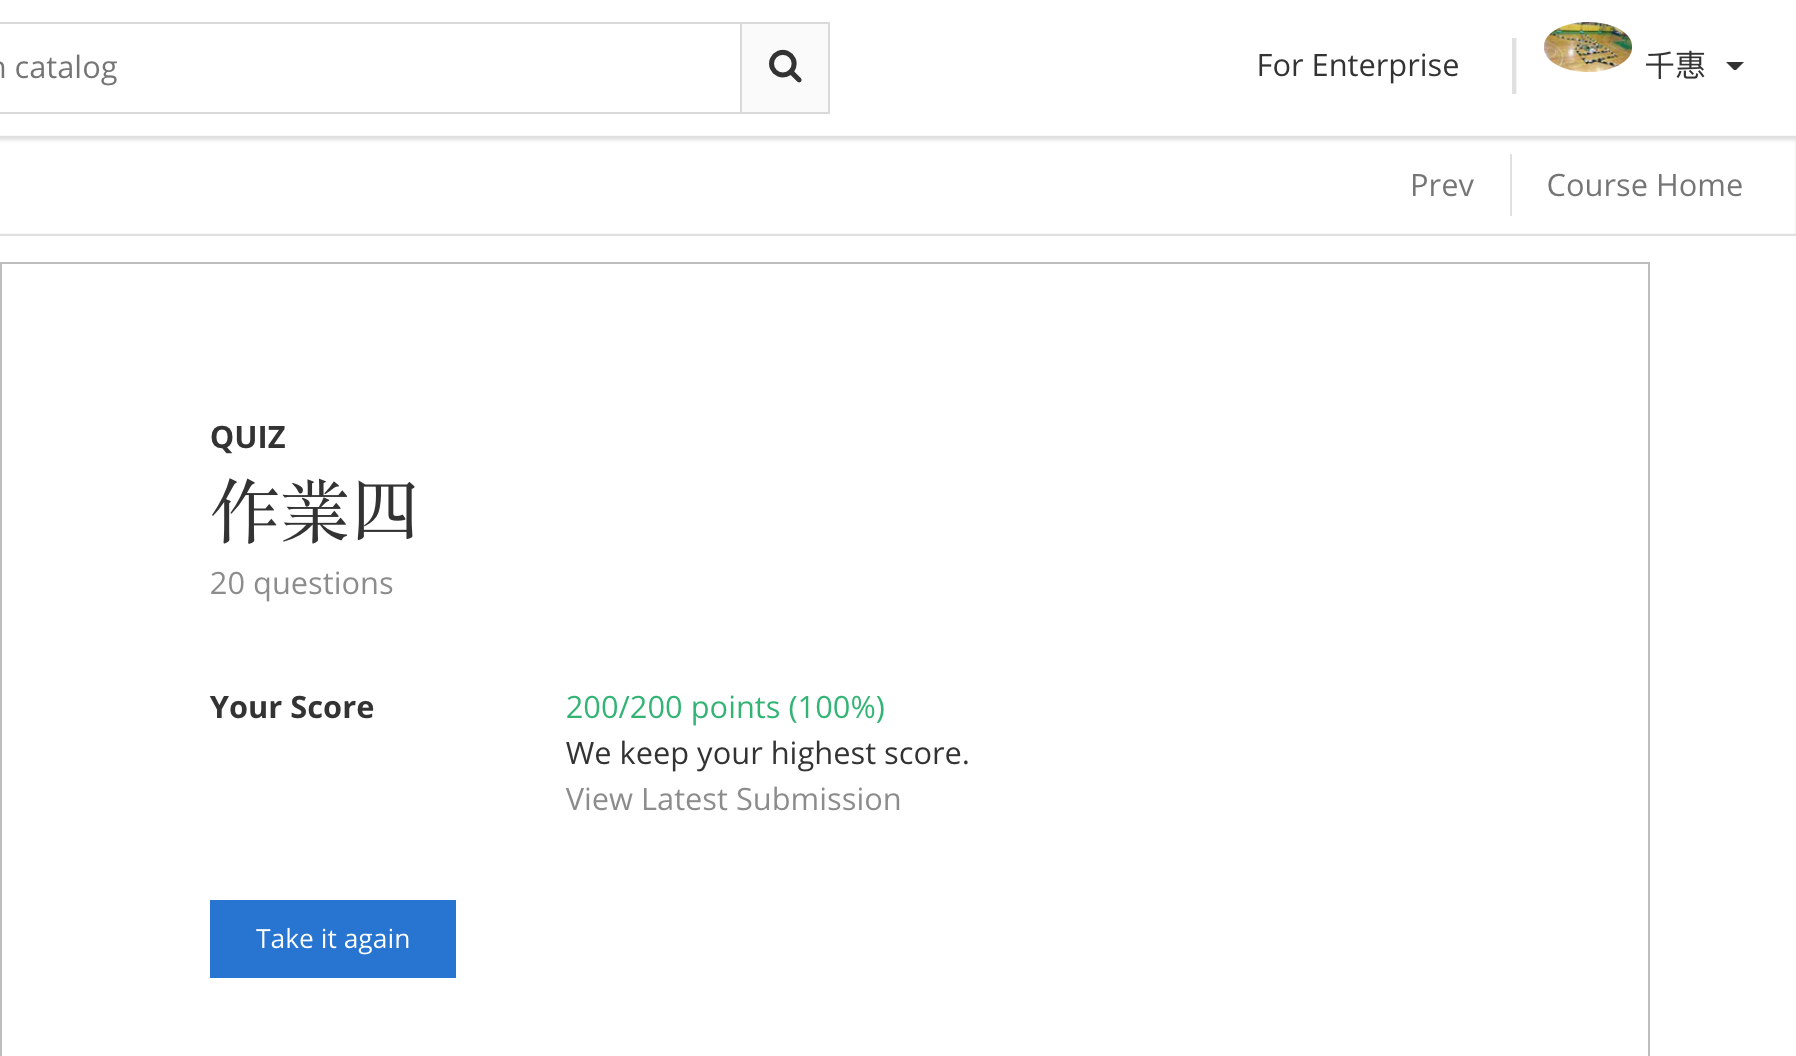
\includegraphics[width=16.5cm, keepaspectratio=true]{1.png}
	
	\section*{Problem 2}
		\vspace{-1em}
		\begin{flalign*} 
			&E_{aug}(\mathbf{w})=E_{in}(\mathbf{w})+\dfrac{\lambda}{N} \mathbf{w}^T\mathbf{w} &\\
			&\Rightarrow\nabla E_{aug}(\mathbf{w}) = \nabla E_{in}(\mathbf{w}) + \dfrac{2\lambda}{N} \mathbf{w} &\\
			&\mathbf{w}(t+1) \leftarrow \mathbf{w}(t) - \eta \nabla E_{aug}(w)&\\
			&\Rightarrow \mathbf{w}(t+1) \leftarrow \mathbf{w}(t) - \eta (\nabla E_{in}(\mathbf{w}) + \dfrac{2\lambda}{N} \mathbf{w})&\\
			&\Rightarrow \mathbf{w}(t+1) \leftarrow (1-\dfrac{2\eta\lambda}{N}) \mathbf{w}(t) - \eta \nabla E_{in}(\mathbf{w}(t))
		\end{flalign*}

	\section*{Problem 3}
		\vspace{-1em}
		\begin{flalign*} 
			&E_{aug}(\mathbf{w})=E_{in}(\mathbf{w})+\dfrac{\lambda}{N} \mathbf{w}^T\mathbf{w} &\\
			&\norm{\mathbf{w}_{reg}(\lambda)}^2 = \mathbf{w}^T\mathbf{w} = C&\\
			&\text{When } \lambda =0 ,\mathbf{w}_{reg}(\lambda) = \mathbf{w}_{lin} \Rightarrow \sqrt C = \norm{\mathbf{w}_{reg}(\lambda)}=\norm{\mathbf{w}_{lin}}&\\
			&\text{Larger } \lambda \Leftrightarrow \text{prefer shorter }\mathbf{w} \Leftrightarrow \text{effectively smaller }C &\\
			&\Rightarrow \text{For any } \lambda > 0, \sqrt C = \norm{\mathbf{w}_{reg}(\lambda)} \leq \norm{\mathbf{w}_{lin}}
		\end{flalign*}

	\section*{Problem 4}
		$E_{loocv} = \dfrac{1}{3}(e_1+e_2+e_3)$
		\begin{enumerate}
		\item Model: constant $h_0(x)=b_0$
			\vspace{-1em}
			\begin{flalign*} 
				&g_1^- = \dfrac{1}{2} \hspace{3em}
				g_2^- = 0  \hspace{3em}
				g_3^- = \dfrac{1}{2} &\\
				&e_1 = err(g_1^-(-1),0) = err(\dfrac{1}{2},0) = (\dfrac{1}{2})^2 = \dfrac{1}{4} &\\
				&e_2 = err(g_2^-(-1),1) = err(0,1) = 1 &\\
				&e_3 = err(g_3^-(-1),0) = err(\dfrac{1}{2},0) = (\dfrac{1}{2})^2 = \dfrac{1}{4} &\\
				&\Rightarrow E_{loocv}(h_0) = \dfrac{1}{3}(\dfrac{1}{4}+1+\dfrac{1}{4})=\dfrac{1}{2}
			\end{flalign*}
		\item Model: linear $h_1(x)=a_1x+b_1$
			\vspace{-1em}
			\begin{flalign*} 
				% &\text{Let }d((x,y), h_1)\text{ be the distance of y from point }(x,y)\text{ to line } h_1. &\\
				&g_1^- = \dfrac{1}{\rho-1}x-\dfrac{1}{\rho-1} \hspace{3em}
				g_2^- = 0  \hspace{3em}
				g_3^- = \dfrac{1}{\rho+1}x+\dfrac{1}{\rho+1} &\\
				&e_1 = err(g_1^-(-1),0) = err(\dfrac{2}{\rho-1}, 0) = (\dfrac{2}{\rho -1})^2 &\\
				&e_2 = err(g_2^-(\rho),1) = err(0,1) = 1 &\\
				&e_3 = err(g_3^-(1),0) = err(\dfrac{2}{\rho+1}, 0) = (\dfrac{2}{\rho+1})^2 &\\
				&\Rightarrow E_{loocv}(h_1) = \dfrac{1}{3}((\dfrac{2}{\rho-1})^2+1+(\dfrac{2}{\rho+1})^2)
			\end{flalign*}
		\end{enumerate}
		\vspace{-1em}
		\begin{flalign*} 
			&E_{loocv}(h_0) = E_{loocv}(h_1) &\\
			&\Rightarrow \dfrac{1}{2} = \dfrac{1}{3}((\dfrac{2}{\rho-1})^2+1+(\dfrac{2}{\rho+1})^2)&\\
			&\Rightarrow \rho = \sqrt{9+4\sqrt{6}}
		\end{flalign*}

	\section*{Problem 5}
		\vspace{-1em}
		\begin{flalign*} 
			&E_{in}(\mathbf{w}_{lin})=\min\limits_{\mathbf{w}}\dfrac{1}{N+K}\Big(\sum_{n=1}^N (y_n-\mathbf{w}^T\mathbf{x}_n) + \sum_{k=1}^{K}(\tilde{y}_k-\mathbf{w}^T\tilde{\mathbf{x}}_k) \Big) &\\
			&E_{in}(\mathbf{w}_{lin})=\min\limits_{\mathbf{w}}\dfrac{1}{N+K}[(\mathbf{w}^T\mathbf{X}^T\mathbf{X}\mathbf{w}+2\mathbf{w}^T\mathbf{X}^T\mathbf{y}+\mathbf{y}^T\mathbf{y}) + (\mathbf{w}^T\tilde{\mathbf{X}}^T\tilde{\mathbf{X}}\mathbf{w}+2\mathbf{w}^T\tilde{\mathbf{X}}^T\tilde{\mathbf{y}}+\tilde{\mathbf{y}}^T\tilde{\mathbf{y}})] &\\
			&\Rightarrow \nabla E_{in}(\mathbf{w}_{lin})= \dfrac{2}{N+K}(\mathbf{X}^T\mathbf{X}\mathbf{w}_{lin}-\mathbf{X}^T\mathbf{y} + \tilde{\mathbf{X}}^T\tilde{\mathbf{X}}\mathbf{w}_{lin}-\tilde{\mathbf{X}}^T\tilde{\mathbf{y}}) = 0&\\
			&\Rightarrow (\mathbf{X}^T\mathbf{X}+\tilde{\mathbf{X}}^T\tilde{\mathbf{X}})\mathbf{w}_{lin}=\mathbf{X}^T\mathbf{y}+\tilde{\mathbf{X}}^T\tilde{\mathbf{y}}&\\
			&\Rightarrow \mathbf{w}_{lin} = (\mathbf{X}^T\mathbf{X}+\tilde{\mathbf{X}}^T\tilde{\mathbf{X}})^{-1}(\mathbf{X}^T\mathbf{y}+\tilde{\mathbf{X}}^T\tilde{\mathbf{y}})
		\end{flalign*}

	\section*{Problem 6}
		\vspace{-1em}
		\begin{flalign*} 
			&\mathbf{w}_{lin} = (\mathbf{X}^T\mathbf{X}+\tilde{\mathbf{X}}^T\tilde{\mathbf{X}})^{-1}(\mathbf{X}^T\mathbf{y}+\tilde{\mathbf{X}}^T\tilde{\mathbf{y}}) &\\
			&\mathbf{w}_{reg}=\argmin\limits_\mathbf{w} \dfrac{\lambda}{N}\norm{\mathbf{w}}^2+\dfrac{1}{N}\norm{\mathbf{X}\mathbf{w}-\mathbf{y}}^2 &\\
			&\Rightarrow \dfrac{2\mathbf{w}_{reg}\lambda}{N}+\dfrac{2}{N}(\mathbf{X}^T\mathbf{X}\mathbf{w}_{reg}-\mathbf{X}^T\mathbf{y})=0&\\
			&\Rightarrow (\lambda\mathbf{I}+\mathbf{X}^T\mathbf{X})\mathbf{w}_{reg}-\mathbf{X}^T\mathbf{y}=0&\\
			&\Rightarrow \mathbf{w}_{reg} = (\mathbf{X}^T\mathbf{X}+\lambda\mathbf{I})^{-1}\mathbf{X}^T\mathbf{y}&\\
			&\mathbf{w}_{lin} = \mathbf{w}_{reg}&\\
			&\Rightarrow \tilde{\mathbf{X}} = \sqrt{\lambda}\mathbf{I}, \tilde{\mathbf{y}} = 0&\\
		\end{flalign*}
	
	\section*{Problem 7}
		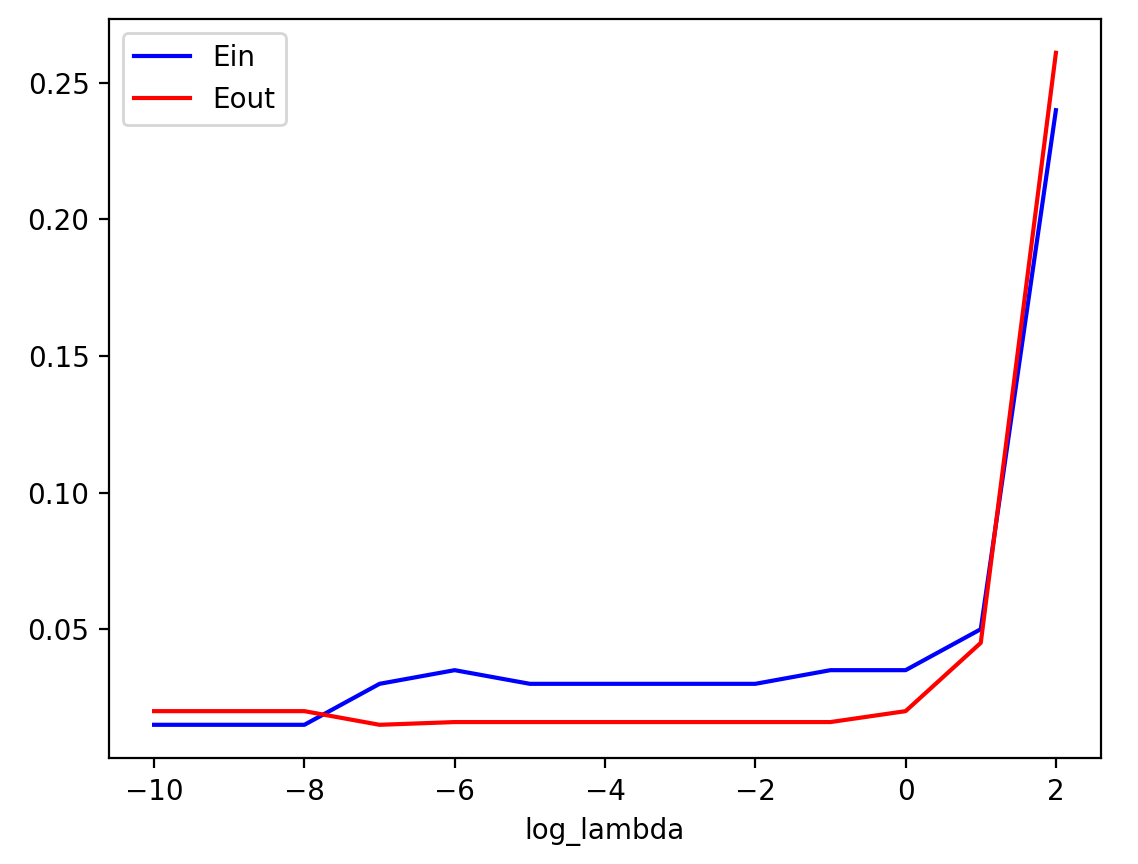
\includegraphics[height=10cm, keepaspectratio=true]{7.png}

	\section*{Problem 8}
		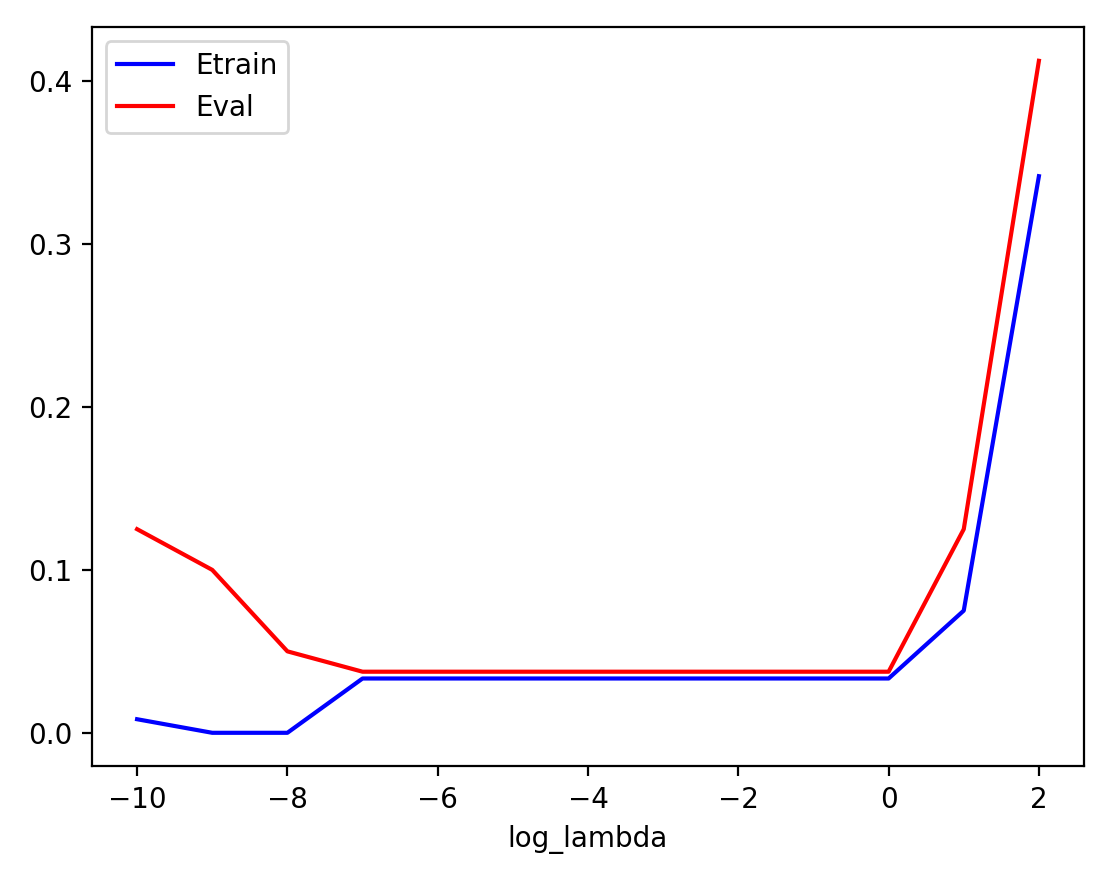
\includegraphics[height=10cm, keepaspectratio=true]{8.png}

	\newpage
	\section*{Problem 9(Bonus)}
		\subsection{}
			\begin{enumerate}
			\item Algorithm $\mathcal{A}_{majority}$
				\vspace{-1em}
				\begin{flalign*} 
					&\text{Let } g\in\mathcal{A}_{majority}, 
					\begin{cases}
					g = +1 \text{ when the majority class is positive}\\
					g = -1 \text{ when the majority class is negative}
					\end{cases}&\\
					&E_{loocv}(\mathcal{A}_{majority})=\dfrac{1}{2252}\sum_{i=1}^{2252} e_i =\dfrac{1}{2252}\sum_{i=1}^{2252} err(g_i^-, y_i)&\\
					&\begin{cases}
					x_i > 0\Rightarrow g_i^- = -1, \hspace{0.5em}y_i = +1 \Rightarrow e_i = 1\\
					x_i < 0\Rightarrow g_i^- = +1, \hspace{0.5em}y_i = -1 \Rightarrow e_i = 1\\
					\end{cases} &\\
					&\Rightarrow E_{loocv}(\mathcal{A}_{majority})= \dfrac{1}{2252}\sum_{i=1}^{2252} 1 = 1
				\end{flalign*}
			\item Algorithm $\mathcal{A}_{minority}$
				\vspace{-1em}
				\begin{flalign*}
					&\text{Let } g\in\mathcal{A}_{minority}, 
					\begin{cases}
					g = +1 \text{ when the minority class is positive}\\
					g = -1 \text{ when the minority class is negative}
					\end{cases}&\\
					&E_{loocv}(\mathcal{A}_{minority})=\dfrac{1}{2252}\sum_{i=1}^{2252} e_i =\dfrac{1}{2252}\sum_{i=1}^{2252} err(g_i^-, y_i)&\\
					&\begin{cases}
					x_i > 0\Rightarrow g_i^- = +1, \hspace{0.5em}y_i = +1 \Rightarrow e_i = 0\\
					x_i < 0\Rightarrow g_i^- = -1, \hspace{0.5em}y_i = -1 \Rightarrow e_i = 0\\
					\end{cases} &\\
					&\Rightarrow E_{loocv}(\mathcal{A}_{minority})= \dfrac{1}{2252}\sum_{i=1}^{2252} 0 = 0
				\end{flalign*}
			\end{enumerate}
			$\Rightarrow \mathcal{A}_{minority}$ algorithm should be chosen if we use $E_{loocv}$ for algorithm selection.
		\newpage
		\subsection{}
			\vspace{-1em}
			\begin{flalign*}
				&\text{Let } g\in\mathcal{A}_{average} \text{ predicts the average value within the data set that it sees.}&\\
				&E_{loocv}(\mathcal{A}_{average})=\dfrac{1}{N}\sum_{i=1}^{N} e_i =\dfrac{1}{N}\sum_{i=1}^{N} err(g_i^-, y_i)&\\
				&\forall x_i, \begin{cases}
				y_i = x_i\\
				g_i^- = \dfrac{N\bar{x}-x_i}{N-1}
				\end{cases} &\\
				&\Rightarrow  err(g_i^-, y_i) = (x_i - \dfrac{N\bar{x}-x_i}{N-1})^2 = (\dfrac{N}{N-1}(x_i-\bar{x}))^2&\\
				&\Rightarrow E_{loocv}(\mathcal{A}_{average})=  \dfrac{N^2}{(N-1)^2}\sum_{i=1}^{N} \dfrac{(x_i-\bar{x})}{N} =  \dfrac{N^2}{(N-1)^2}\sum_{i=1}^{N} \dfrac{(y_i-\bar{y})}{N} = \dfrac{N^2}{(N-1)^2} \mathrm{Var}\left[\{y_n\}_{n=1}^N\right]&\\
				&\Rightarrow E_{loocv}(\mathcal{A}_{average}) \text{ is a scaled version of the variance of } \{y_n\}_{n=1}^N
			\end{flalign*}

	\clearpage
	\end{CJK}
\end{document}